\chapter{Anhang}


\begin{figure}[H]
\begin{minted}{json}
    
{
"type": "MESSAGE",
"eventTime": "2024-07-04T18:57:11.735759Z",
"message": {
    "name": "spaces/****/messages/****",
    "sender": {
        "name": "users/****",
        "displayName": "Atakan Sentürk",
        "avatarUrl": "https://lh3.googleusercontent.com/a/**",
        "email": "a.sentuerk@****.de",
        "type": "HUMAN",
        "domainId": "****"
    },
    "createTime": "2024-07-04T18:57:11.735759Z",
    "text": "@Arthur Hi",
    "annotations": [
        {
            "type": "USER_MENTION",
            "startIndex": 0,
            "length": 7,
            "userMention": {
            "user": {
                "name": "users/****",
                "displayName": "Arthur",
                "avatarUrl": "https://lh5.googleusercontent.com/**",
                "type": "BOT"
            },
            "type": "MENTION"
            }
        }
    ],
    "thread": {
        "name": "spaces/****/threads/****",
        "retentionSettings": {
            "state": "PERMANENT"
    }
    },
    "space": {
        "name": "spaces/****",
        "type": "ROOM",
        "displayName": "Bot Test",
        "spaceThreadingState": "THREADED_MESSAGES",
        "spaceType": "SPACE",
        "spaceHistoryState": "HISTORY_ON",
        "spaceUri": "https://chat.google.com/room/**?cls=11"
\end{minted}
\end{figure}
\begin{figure}[H]
    \ContinuedFloat
                \begin{minted}{json}
    },
    "argumentText": " Hi",
    "threadReply": true,
    "retentionSettings": {
        "state": "PERMANENT"
    },
    "messageHistoryState": "HISTORY_ON",
    "formattedText": "@Arthur Hi"
},
"user": {
    "name": "users/****",
    "displayName": "Atakan Sentürk",
    "avatarUrl": "https://lh3.googleusercontent.com/a/**",
    "email": "a.sentuerk@****.de",
    "type": "HUMAN",
    "domainId": "****"
},
"space": {
    "name": "spaces/****",
    "type": "ROOM",
    "displayName": "Bot Test",
    "spaceThreadingState": "THREADED_MESSAGES",
    "spaceType": "SPACE",
    "spaceHistoryState": "HISTORY_ON",
    "spaceUri": "https://chat.google.com/room/***?cls=11"
},
"configCompleteRedirectUrl": "https://chat.google.com/api/**",
"common": {
    "userLocale": "de",
    "hostApp": "CHAT"
}
}
\end{minted}
\caption{JSON Objekt, welches der Chatbot von der API erhält}
\label{msg_get}
\end{figure}

\begin{figure}[H]
\begin{minted}{python}
{
    parent=req["message"]["space"]["name"],
    messageReplyOption='REPLY_MESSAGE_FALLBACK_TO_NEW_THREAD',
    
    body=
    {
        "text": "<"+user["name"]+"> "+ans["answer"], 
        "thread": {"name": thread_name}
    }
}
\end{minted}
\caption{Message Objekt, welches asynchron als Antwort an die API gesendet wird}
\label{msg_send}
\end{figure}
\begin{figure}[t]
    \centering
    \includegraphics[width=\linewidth]{\figdir/Chat}
    \caption{Darstellung des Google Chats und eines Threads}
    \label{chat}
\end{figure}
\begin{figure}[t]
    \centering
    \includegraphics[width=\linewidth]{\figdir/Thread}
    \caption{Darstellung der Erinnerung an alte Nachrichten innerhalb eines Threads}
    \label{thread}
\end{figure}
\begin{figure}
    \centering
    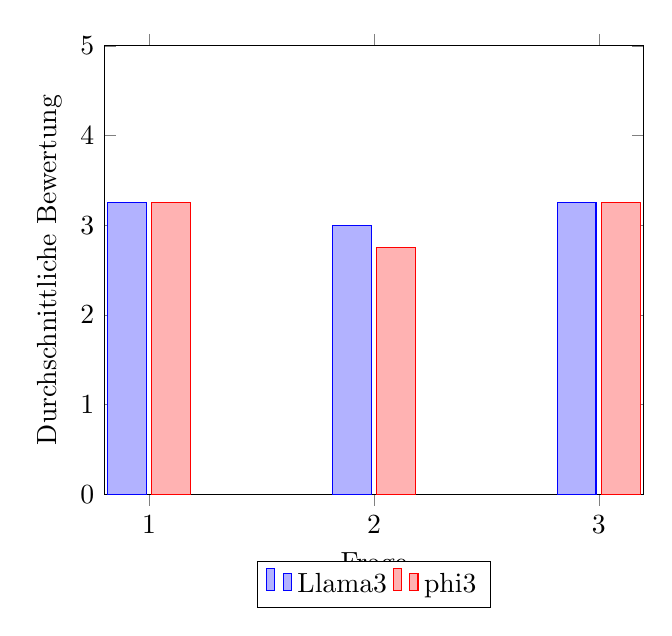
\begin{tikzpicture}
        
    \begin{axis}[
        ybar,
        bar width=14pt,
        ylabel={Durchschnittliche Bewertung},
        xlabel={Frage},
        ymin=0,
        ymax=5,
        symbolic x coords={1,2,3},
        xtick=data,
        legend style={at={(0.5,-0.15)},
        anchor=north,legend columns=-1},
        ylabel near ticks,
        xlabel near ticks
    ]
    \addplot coordinates {(1,3.25) (2,3) (3,3.25)};
    \addplot coordinates {(1,3.25) (2, 2.75) (3,3.25)};
    \legend{Llama3 , phi3}
    \end{axis}
    \end{tikzpicture}
    \caption{Bewertungen von Llama3 und Phi3}
    \label{bewertung}
\end{figure}

\begin{figure}[t]
    \centering
    \includegraphics[width=\linewidth]{\figdir/stars}
    \caption{Github Star Historie von den Frameworks Langchain, Haystack und LlamaIndex}
    \label{stars}
    \end{figure}
%%% Local Variables: 
%%% mode: latex
%%% TeX-master: "thesis.tex"
%%% End: 
